\documentclass[12pt,]{article}
\usepackage[utf8]{inputenc}
\usepackage[T1]{fontenc}
\usepackage{mathptmx}
\usepackage{geometry}
\usepackage{mathtools}
\usepackage[english]{babel}
\usepackage{graphicx}
\usepackage{stackengine}
\usepackage[os=win]{menukeys}
\usepackage{hyperref}
\usepackage{minted}
\usepackage{xcolor}
\usepackage{tikz}
\usepackage[yyyymmdd,hhmmss]{datetime}
\usepackage{etoolbox}
\usepackage[inline]{enumitem}

\newcommand{\WindowsLogo}{\raisebox{-0.1em}{
\includegraphics[height=0.8em]{images/logo/Windows_3_logo_simplified}}}
%\newcommand{\PowerLogo}{\raisebox{-0.1em}{
\includegraphics[height=0.8em]{images/logo/power}}}
\newcommand{\WinKey}{\keys{\WindowsLogo}}       
\newcommand{\PowerKey}{\keys{\PowerLogo}}       

\patchcmd{\thebibliography}{\section*{\refname}}{}{}{}

\newcommand{\ShowOsVersion}{
        \immediate\write18{\unexpanded{foo=`uname -sro` && echo "${foo}" > tmp.tex}}
        \input{tmp}\immediate\write18{rm tmp.tex}
}

\newcommand{\ShowTexVersion}{
        \immediate\write18{\unexpanded{foo=`pdflatex -version | head -n1 | cut -d' ' -f1,2` && echo "${foo}" > tmp.tex}}
        \input{tmp}\immediate\write18{rm tmp.tex}
}

\addto\captionsenglish{\renewcommand{\contentsname}{Daftar Isi}}
\addto\captionsenglish{\renewcommand{\figurename}{Gambar}}

\hypersetup{
        colorlinks=true, %set true if you want colored links
        linktoc=all,     %set to all if you want both sections and subsections linked
        linkcolor=blue,  %choose some color if you want links to stand out
        urlcolor=blue,   %url color
}

\geometry{
        a4paper,
        left=15mm,
        right=10mm,
        top=10mm,
        bottom=15mm,
}

\title{\LARGE \bf
        Panduan Pengujian Lanjutan\\
        \small{(Handheld Audiometri Prototype)}
}

\author{Achmadi ST MT}

\date{}

\hypersetup{citecolor=black}

\definecolor{LightGray}{gray}{0.95}

%\pagecolor[rgb]{0.1,0.1,0.1}
%\color[rgb]{1,1,1}

\begin{document}
	\thispagestyle{empty}
	
	\begin{titlepage}
		\centering
		\vfill
		\vfill
		\maketitle
		\vfill
		
\includegraphics[width=200pt]{images/logo/logoviblab}
		\vfill
		\vfill
		Update: {\today} \currenttime \\
	\end{titlepage}
	
	%%%%%%%%%%%%%%%%%%%%%%%%%%%%%%%%%%%%%%%%%%%%%%%%%%%%%%%%%%%%%%%%%
	
	\newpage
	\tableofcontents
	
	%%%%%%%%%%%%%%%%%%%%%%%%%%%%%%%%%%%%%%%%%%%%%%%%%%%%%%%%%%%%%%%%%
	
	\newpage
	\section{Pendahuluan}
	
	\subsection{Hasil Sebelumnya}
	
	Berikut ditampilkan rangkuman dari hasil pengukuran sebelumnya:
	
	\subsubsection{Headphone BOSE}
	
	Berikut tabel nilai (dalam dB-SPL) dan respon Sine-Sweep.
	Nilai didapat dari pengukuran berulang dengan diambil nilai paling sering muncul.
	
	Hasil dari Prototype Box-1 (dB-SPL):
	
	\begin{center}
		\begin{tabular}{|l|l|l|l|l|l|l|l|l|l|}
			\hline
			\textbf{Fq/Amp}  & \textbf{9} & \textbf{8} & \textbf{7} & \textbf{6} & \textbf{5} & \textbf{4} & \textbf{3} & \textbf{2} & \textbf{1} \\ \hline
			\textbf{250 Hz}  & 75.0       & 68.9       & 62.8       & 56.8       & 50.7       & 45.1       & 40.2       & 35.4       & 32.5       \\ \hline
			\textbf{500 Hz}  & 74.5       & 68.4       & 62.4       & 56.3       & 50.3       & 44.5       & 39.4       & 35.1       & 31.5       \\ \hline
			\textbf{1000 Hz} & 81.2       & 75.2       & 69.2       & 63.1       & 57.1       & 51.2       & 45.5       & 40.8       & 37.2       \\ \hline
			\textbf{2000 Hz} & 78.0       & 71.9       & 65.9       & 59.8       & 53.8       & 48.2       & 42.7       & 38.2       & 35.2       \\ \hline
			\textbf{4000 Hz} & 82.9       & 76.9       & 70.9       & 64.8       & 58.8       & 53.0       & 47.8       & 43.8       & 41.0       \\ \hline
			\textbf{8000 Hz} & 79.1       & 73.0       & 67.0       & 60.9       & 55.2       & 49.6       & 45.4       & 42.8       & 42.0       \\ \hline
		\end{tabular}
	\end{center}

	Hasil dari Prototype Box-2 (dB-SPL):
	
	\begin{center}
		\begin{tabular}{|l|l|l|l|l|l|l|l|l|l|}
			\hline
			\textbf{Fq/Amp}  & \textbf{9} & \textbf{8} & \textbf{7} & \textbf{6} & \textbf{5} & \textbf{4} & \textbf{3} & \textbf{2} & \textbf{1} \\ \hline
			\textbf{250 Hz}  & 76.1       & 70.1       & 64.1       & 58.0       & 52.1       & 46.3       & 41.2       & 37.6       & 36.2       \\ \hline
			\textbf{500 Hz}  & 75.1       & 69.1       & 63.0       & 56.9       & 50.1       & 45.3       & 41.0       & 36.5       & 33.6       \\ \hline
			\textbf{1000 Hz} & 80.8       & 74.8       & 68.8       & 62.7       & 56.6       & 50.8       & 45.5       & 41.1       & 38.1       \\ \hline
			\textbf{2000 Hz} & 76.9       & 70.8       & 64.8       & 58.7       & 52.7       & 47.1       & 42.2       & 39.0       & 37.4       \\ \hline
			\textbf{4000 Hz} & 83.2       & 77.2       & 71.2       & 65.1       & 59.2       & 53.4       & 48.1       & 43.9       & 41.2       \\ \hline
			\textbf{8000 Hz} & 77.4       & 71.5       & 65.4       & 59.4       & 53.7       & 48.5       & 44.4       & 42.3       & 41.5       \\ \hline
		\end{tabular}
	\end{center}

	Respon Sine-Sweep:
	
	\begin{figure}[!ht]
		\centering
		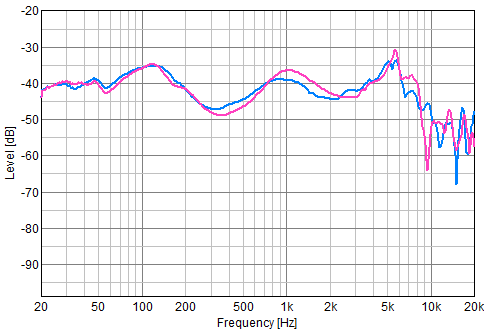
\includegraphics[width=300pt]{images/respon/FP-Bose}
		\caption{Respon Sine-Sweep BOSE}
	\end{figure}

	\newpage
	\subsubsection{Headphone Miniso}
	
	Berikut tabel nilai (dalam dB-SPL) dan respon Sine-Sweep.
	Nilai didapat dari pengukuran berulang dengan diambil nilai paling sering muncul.
	
	Hasil dari Prototype Box-1 (dB-SPL):
	
	\begin{center}
		\begin{tabular}{|l|l|l|l|l|l|l|l|l|l|}
			\hline
			\textbf{Fq/Amp}  & \textbf{9} & \textbf{8} & \textbf{7} & \textbf{6} & \textbf{5} & \textbf{4} & \textbf{3} & \textbf{2} & \textbf{1} \\ \hline
			\textbf{250 Hz}  & 73.7       & 67.7       & 61.7       & 55.7       & 49.9       & 44.1       & 38.7       & 33.7       & 30.5       \\ \hline
			\textbf{500 Hz}  & 74.8       & 68.8       & 62.9       & 56.9       & 51.0       & 45.2       & 39.8       & 34.9       & 31.1       \\ \hline
			\textbf{1000 Hz} & 78.0       & 72.0       & 66.0       & 60.1       & 54.2       & 48.4       & 43.0       & 38.0       & 34.3       \\ \hline
			\textbf{2000 Hz} & 68.7       & 62.6       & 56.7       & 50.7       & 44.9       & 39.1       & 34.0       & 29.9       & 27.2       \\ \hline
			\textbf{4000 Hz} & 62.2       & 56.2       & 50.2       & 44.3       & 38.7       & 33.6       & 29.6       & 27.7       & 27.0       \\ \hline
			\textbf{8000 Hz} & 65.0       & 59.0       & 53.0       & 47.2       & 41.5       & 36.3       & 32.7       & 30.4       & 29.6       \\ \hline
		\end{tabular}
	\end{center}
	
	Hasil dari Prototype Box-2 (dB-SPL):
	
	\begin{center}
		\begin{tabular}{|l|l|l|l|l|l|l|l|l|l|}
			\hline
			\textbf{Fq/Amp}  & \textbf{9} & \textbf{8} & \textbf{7} & \textbf{6} & \textbf{5} & \textbf{4} & \textbf{3} & \textbf{2} & \textbf{1} \\ \hline
			\textbf{250 Hz}  & 85.2       & 79.2       & 73.2       & 67.2       & 61.2       & 55.3       & 49.7       & 45.3       & 41.6       \\ \hline
			\textbf{500 Hz}  & 86.4       & 80.4       & 74.4       & 68.4       & 62.4       & 56.5       & 51.1       & 46.1       & 42.3       \\ \hline
			\textbf{1000 Hz} & 89.7       & 83.7       & 77.7       & 71.7       & 65.8       & 59.9       & 54.3       & 49.3       & 45.5       \\ \hline
			\textbf{2000 Hz} & 80.1       & 74.0       & 68.0       & 62.0       & 56.0       & 50.2       & 45.1       & 41.0       & 38.7       \\ \hline
			\textbf{4000 Hz} & 73.7       & 67.7       & 61.7       & 55.7       & 49.9       & 44.8       & 41.0       & 39.0       & 38.4       \\ \hline
			\textbf{8000 Hz} & 76.0       & 70.1       & 64.1       & 58.1       & 52.4       & 47.3       & 43.9       & 42.0       & 41.5       \\ \hline
		\end{tabular}
	\end{center}
	
	Respon Sine-Sweep:
	
	\begin{figure}[!ht]
		\centering
		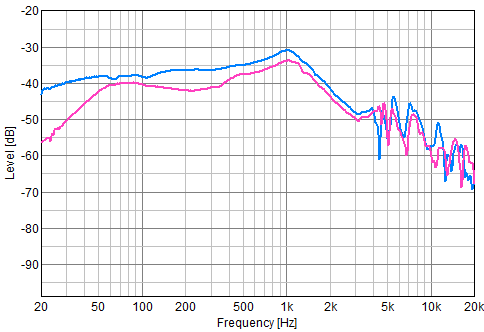
\includegraphics[width=300pt]{images/respon/FP-Miniso}
		\caption{Respon Sine-Sweep Miniso}
	\end{figure}

	\newpage
	\subsection{Belum Terukur}
	
	Berikut adalah poin yang belum terukur sehingga diperlukan pengukuran lanjut:
	\begin{enumerate}
		\item \textbf{Background}.\\
		Untuk mendapatkan hasil ukur yang dipercaya, maka perlu diukur kondisi lingkungan pengukuran.
		Dalam hal ini adalah pengukuran bising ruang pengukuran.
		Hasil ukur bising ini akan jadi acuan pembanding hasil ukur akhir pada nantinya.
		
		\item \textbf{Konsistensi}.\\
		Sebagai salah satu poin penting dalam pengembangan prototype adalah konsistensi unit.
		Ketidak-konsistensi yang dapat timbul antara lain:
		\begin{itemize}
			\item Pemasangan Headphone yang berubah.
			\item Daya baterai yang berubah sehingga suplay arus berubah.
			\item Efek histeresis akibat induktor filter output atau impedansi headphone.
		\end{itemize}
		
	\end{enumerate}

	\newpage
	\section{Pengecekan}
	
	\subsection{PENTING}
	
	Sebelum melanjutkan pengukuran, diperlukan pengecekan kondisi unit prototype,
	mengingat prototype merupakan \textit{hand-made} yang belum reliable untuk ditinggalkan dalam
	kondisi tanpa pengawasan dalam jangka waktu lama.
	
	Beberapa poin yang perlu dilakukan pengecekan unit:
	\begin{itemize}
		\item Unit masih bisa menyala.
		\item Unit tidak mengeluarkan asap saat dinyalakan.
		\item LED biru sebagai indikator masih menyala dan berkedip.
		\item Pasang Headphone, kemudian matikan dan nyalakan kembali unit. Sesaat setelah menyala
		akan dihasilkan nada murni 500Hz sebanyak dua kali bergantian kanan dan kiri.
	\end{itemize}
	
	Jika muncul kegagalan (\textit{failure}) dari salah satu poin di atas maka pengukuran tidak bisa dilakukan
	dan unit prototype harus kembali (\textit{return to base}).
	
	\newpage
	\section{Panduan}
	
	Berikut adalah panduan ringkas pengukuran.
	Panduan sama dengan dokumen panduan sebelumnya namun tanpa \textit{charging} dan beberapa tambahan terkait poin yang belum terukur.
	
	\subsection{Persiapan}
	
	\subsubsection{Hardware}
	
	Berikut adalah perangkat keras yang perlu disiapkan untuk pengujian ini:
	\begin{enumerate}
		\item Unit Prototype Audiometri yang akan diuji.
		Pastikan unit prototype masih normal sebagaimana pada bab sebelumnya.
		\begin{figure}[!ht]
			\centering
			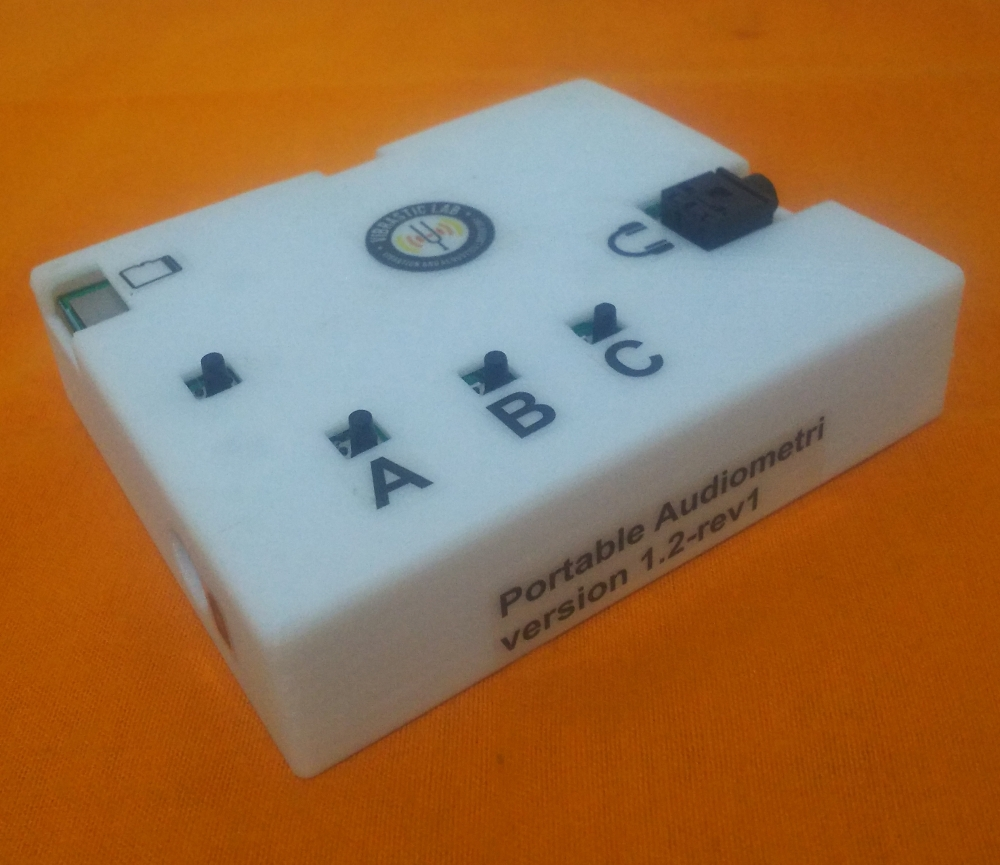
\includegraphics[width=150pt]{images/foto/unit}
			\caption{Unit Prototype}
		\end{figure}
		
		\item Kabel Micro-USB ke USB-A.
		\begin{figure}[!ht]
			\centering
			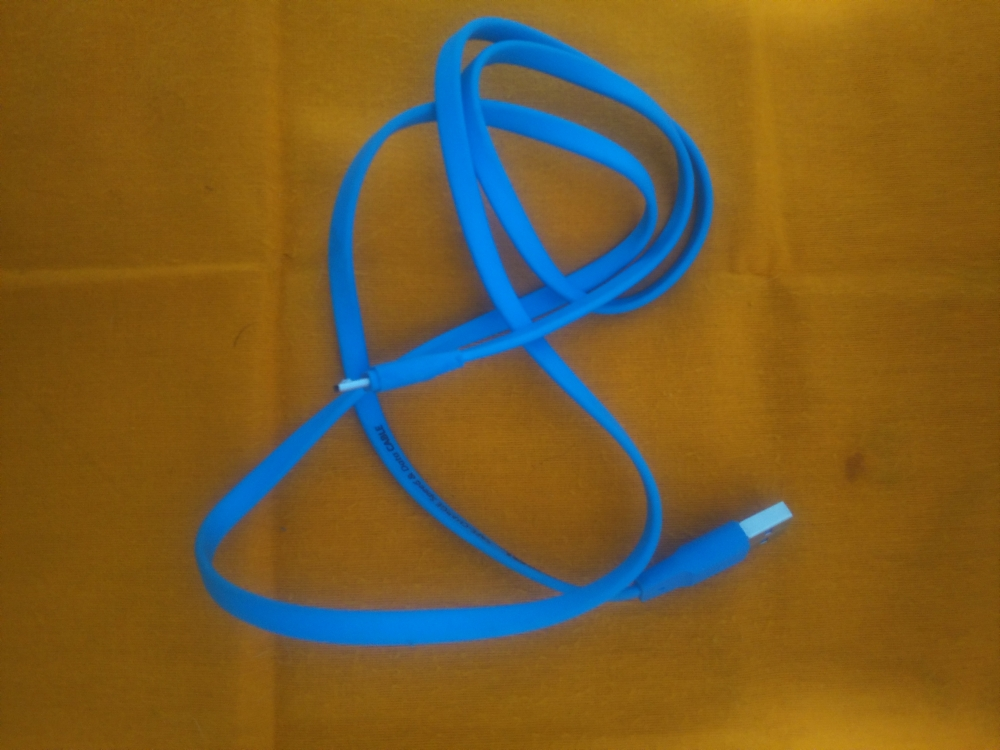
\includegraphics[width=150pt]{images/foto/kabel}
			\caption{Kabel USB}
		\end{figure}
		
		\item Wired-Headphone dengan impedansi tiap channel antara $32\Omega$ hingga $300\Omega$
		\begin{figure}[!ht]
			\centering
			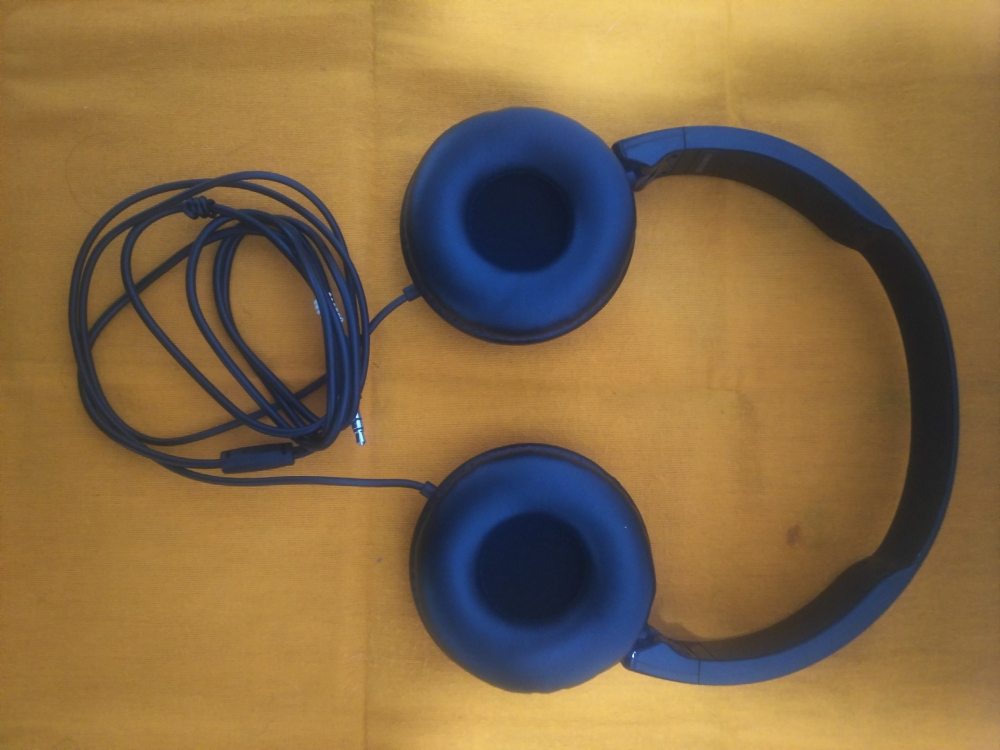
\includegraphics[width=150pt]{images/foto/phone}
			\caption{Wired Headphone}
		\end{figure}
		
		\newpage
		\item Setup Uji KEMAR dan telah terkalibrasi.\\
		\textbf{Catatan}: Diasumsikan bahwa operator telah cukup familiar dalam detil teknis persiapan
		maupun penggunaan unit uji KEMAR.
		\begin{figure}[!ht]
			\centering
			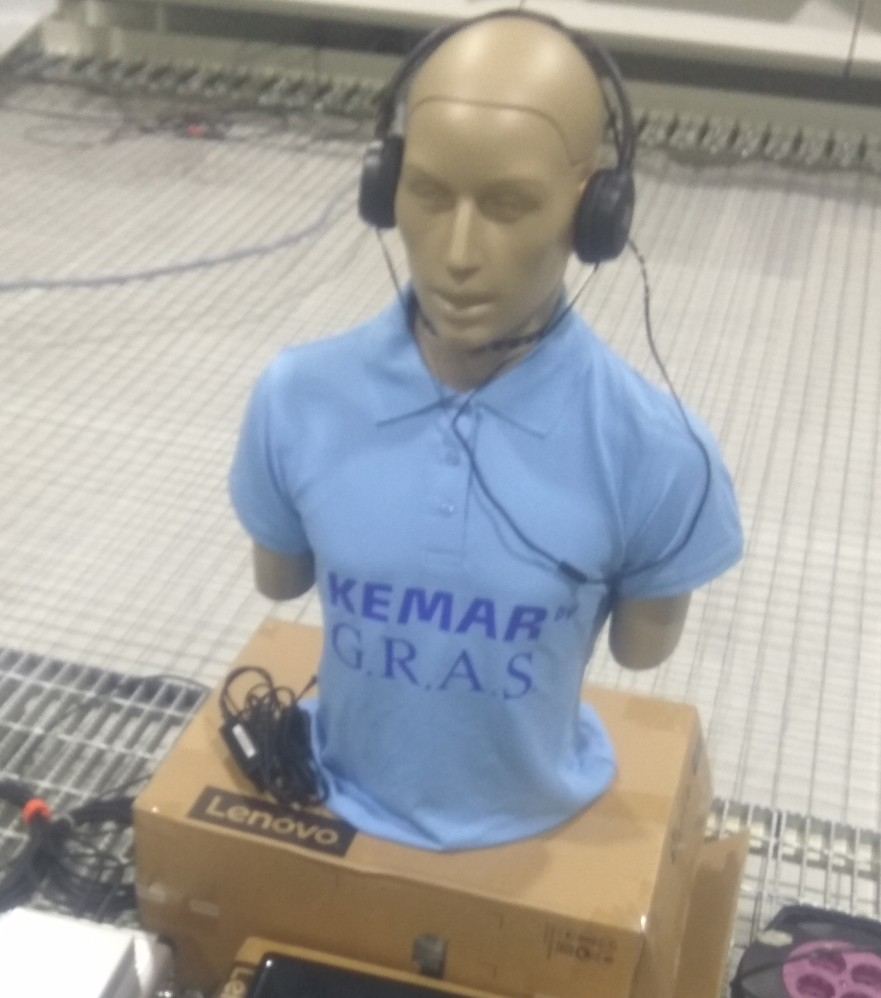
\includegraphics[width=150pt]{images/foto/kemar}
			\caption{Setup Kemar}
		\end{figure}
		
	\end{enumerate}
	
	\subsubsection{Software: Windows}
	
	Berikut adalah perangkat lunak yang perlu disiapkan untuk pengujian ini
	(panduan ini menggunakan Windows-7 32-bit sebagai contoh):
	
	\begin{enumerate}
		\item Install driver ARM USB-CDC.\\
		Untuk dapat menghubungkan unit prototype dengan komputer,
		diperlukan driver ARM USB-CDC untuk komunikasi serial.
		
		\begin{itemize}
			\item File installer (sesuaikan dengan bit OS).
			Dapat didownload di \url{http://intip.in/stm32tools}
			\begin{figure}[!ht]
				\centering
				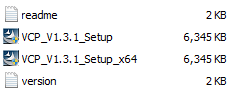
\includegraphics[width=200pt]{images/terminal/driver}
				\caption{Installer Driver}
			\end{figure}
			
			\item Instalasi driver (tanpa unit prototype terhubung) cukup mudah sebagaimana umumnya.
			\begin{figure}[!ht]
				\centering
				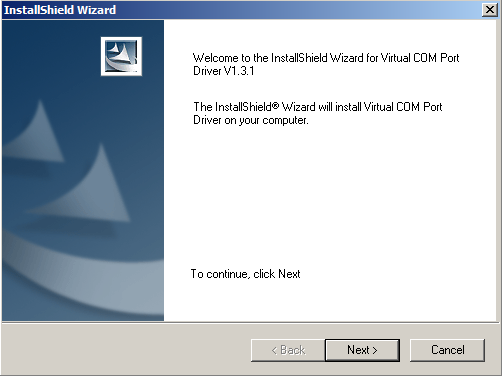
\includegraphics[width=200pt]{images/terminal/install_driver}
				\caption{Mulai instal driver}
			\end{figure}
		\end{itemize}
		
		\newpage
		\item Nyalakan dan hubungkan unit ke komputer.\\
		
		Berikut langkah-langkahnya:
		\begin{itemize}
			\item Hidupkan dengan switch pada sisi samping casing.
			\begin{figure}[!ht]
				\centering
				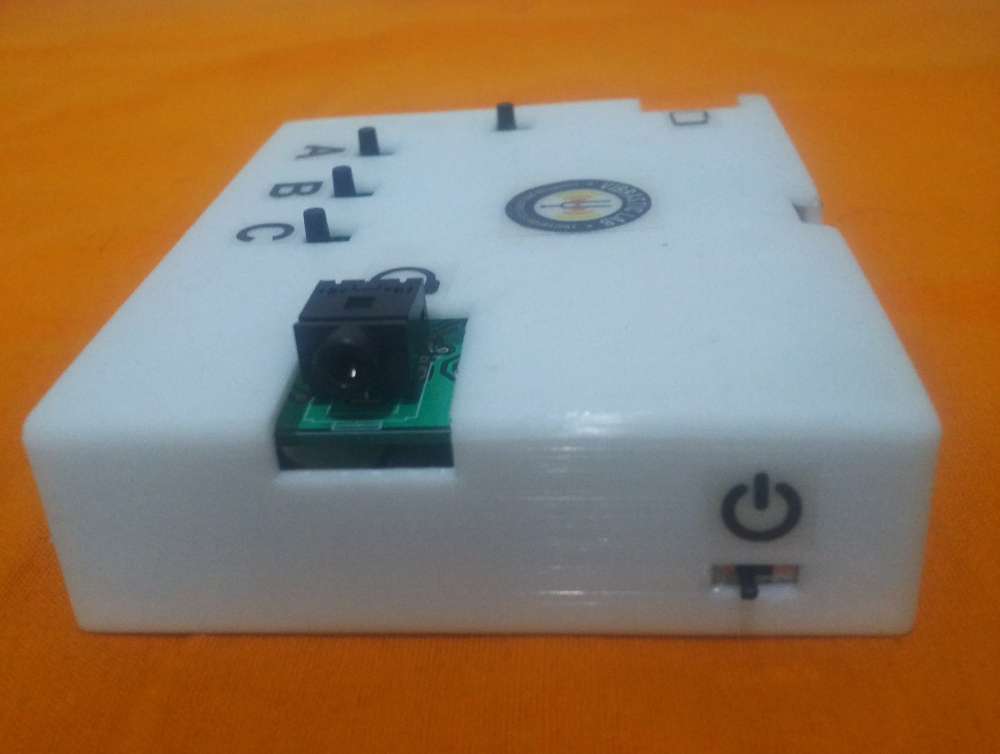
\includegraphics[width=150pt]{images/foto/pwrsw}
				\caption{Power Switch}
			\end{figure}
			
			\item Tunggu hingga LED biru, hijau, dan merah menyala
			bergantian sebagai tanda unit sudah standby
			
			\begin{figure}[!ht]
				\centering
				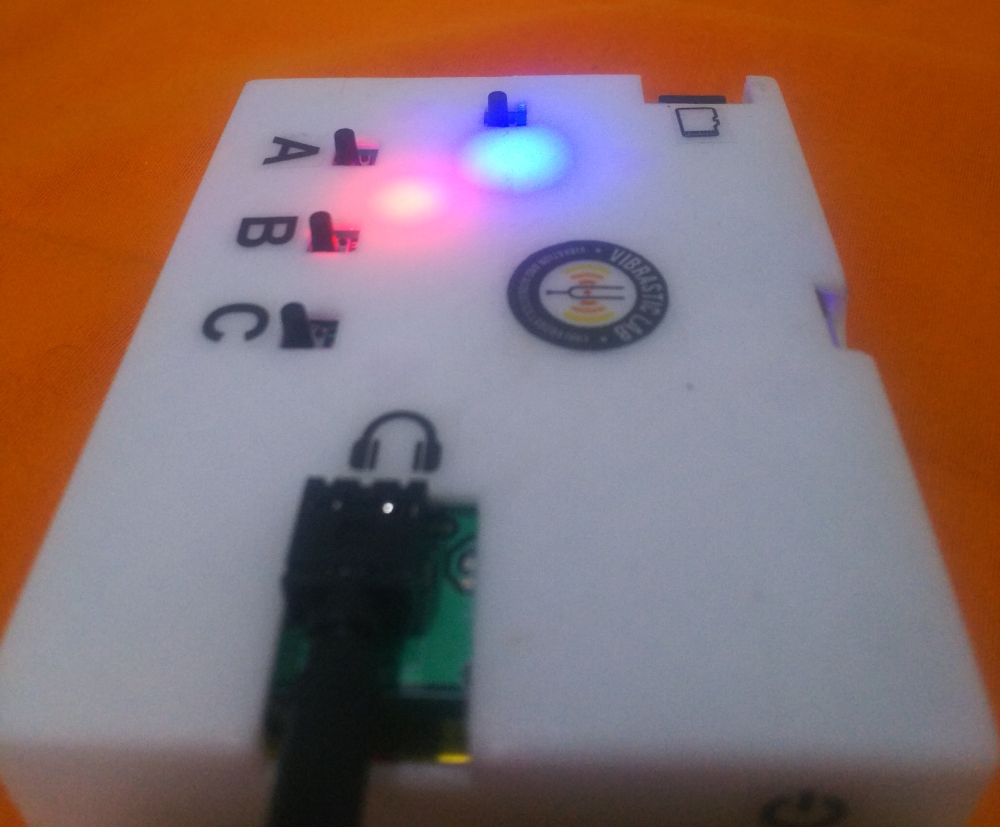
\includegraphics[width=150pt]{images/foto/standby}
				\caption{Unit Standby}
			\end{figure}
			
			\item Sambungkan unit prototype dengan komputer via kabel USB.
			
			\begin{figure}[!ht]
				\centering
				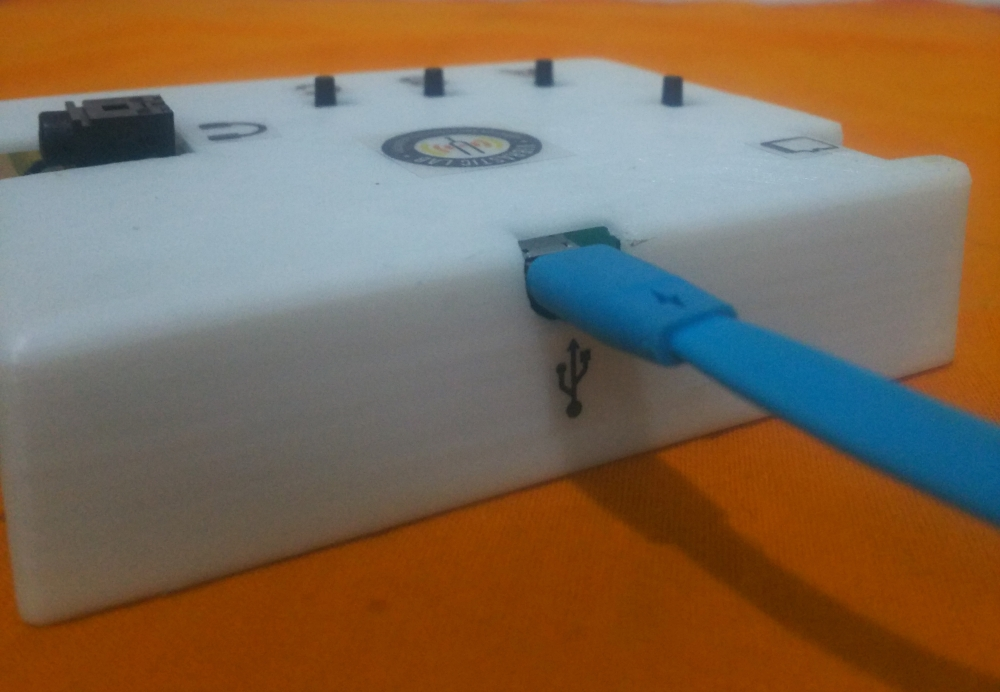
\includegraphics[width=150pt]{images/foto/konek}
				\caption{Konek Kabel USB}
			\end{figure}
			
		\end{itemize}
		
		\newpage
		\item Tunggu hingga driver selesai mengkonfigurasi otomatis
		
		\item Cek \textit{Device Manager} untuk mengetahui Nomor Serial-Port
		\begin{itemize}
			\item Buka run-command dialog dengan kombinasi keyboard (\keys{\WinKey + r})
			
			\item masukkan perintah \textbf{devmgmt.msc}.
			\begin{figure}[!ht]
				\centering
				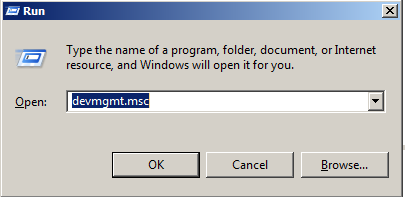
\includegraphics[width=200pt]{images/terminal/devicemgr}
				\caption{Memanggil Device Manager}
			\end{figure}
			
			\item Tekan (\keys{\return}) atau klik OK
			
			\item Cari entry \textit{Ports (COM and LPT)}.
			Catat nomor port untuk entry \textit{STMicroelectronics Virtual COM Port}.
			Dalam contoh ini, terkonfigurasi pada COM3.
			
			\begin{figure}[!ht]
				\centering
				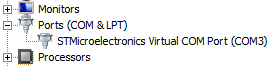
\includegraphics[width=200pt]{images/terminal/comport}
				\caption{Serial Komunikasi pada COM3}
			\end{figure}
		\end{itemize}
		
		\item Install Serial Terminal.
		Untuk dapat berkomunikasi via serial port, perlu diinstall serial terminal.
		Disini dicontohkan menggunakan \textit{Hercules}.
		
		\begin{itemize}
			\item Program terminal Hercules. Dapat didownload di \url{http://intip.in/stm32tools}
			\begin{figure}[!ht]
				\centering
				
\includegraphics[width=200pt]{images/terminal/hercules}
				\caption{Hercules Terminal}
			\end{figure}
			
			\item Jalankan program Hercules.
			Jika muncul konfirmasi lisensi, cukup \textit{Close} saja.
			
			\item Pilih tab \textit{Serial}.
			\begin{figure}[!ht]
				\centering
				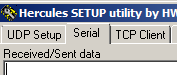
\includegraphics[width=200pt]{images/terminal/hercules_serial}
				\caption{Serial Terminal}
			\end{figure}
			
		\end{itemize}
		
		\newpage
		\item Test Komunikasi Serial
		\begin{itemize}
			\item Hercules Serial Terminal
			\begin{figure}[!ht]
				\centering
				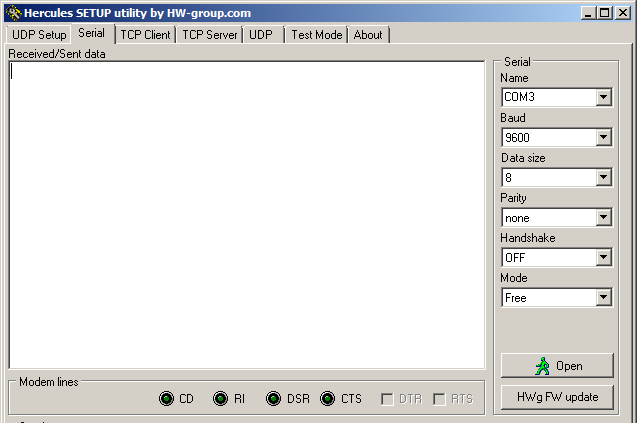
\includegraphics[width=250pt]{images/terminal/hercules_terminal}
				\caption{Hercules Serial Terminal}
			\end{figure}
			
			\item Setting Port pada Serial Terminal sebagai berikut
			\begin{itemize}
				\item Name     : COM3
				\item Baud     : 9600
				\item Data size: 8
				\item Parity   : none
			\end{itemize}
			
			\begin{figure}[!ht]
				\centering
				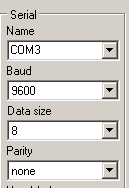
\includegraphics[width=100pt]{images/terminal/hercules_port}
				\caption{Pengaturan serial port}
			\end{figure}
			
			\item Klik Open (pastikan unit prototype sudah standby dan terhubung
			serta nama COM port sudah sesuai)
			
			\begin{figure}[!ht]
				\centering
				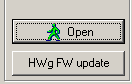
\includegraphics[width=100pt]{images/terminal/hercules_open}
				\caption{Open Serial Port}
			\end{figure}
			
			\item Kolom terminal akan menampilkan pesan:
			\begin{minted}[frame=lines,framesep=2mm,fontsize=\small]{text}
			Serial port COM3 opened
			\end{minted}
			
			\newpage
			\item Selanjutnya, pada kolom terminal,
			masukkan perintah berikut dan diakhiri dengan (\keys{\return})
			\begin{minted}[frame=lines,framesep=2mm,fontsize=\small]{text}
			info
			\end{minted}
			Serial akan menampilkan informasi kernel dan platform
			\begin{figure}[!ht]
				\centering
				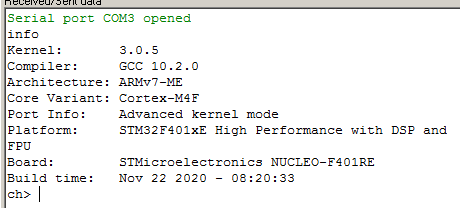
\includegraphics[width=300pt]{images/terminal/hercules_text}
				\caption{Informasi Platform}
			\end{figure}
		\end{itemize}
	\end{enumerate}
	
	\subsubsection{Audio Analyzer}
	
	Untuk perangkat lunak Audio Analyzer, digunakan program \textit{Real-Time Analyzer}
	yang merupakan bagian dari paket software DSFF3 buatan Yoshimasha.
	Jika membutuhkan versi trial dapat didownload di \url{http://intip.in/stm32tools}.
	
	Antar-muka Real-Time Analyzer yang digunakan adalah \textit{FFT-Analyzer} pada tab \textit{Octave band}.
	
	\begin{figure}[!ht]
		\centering
		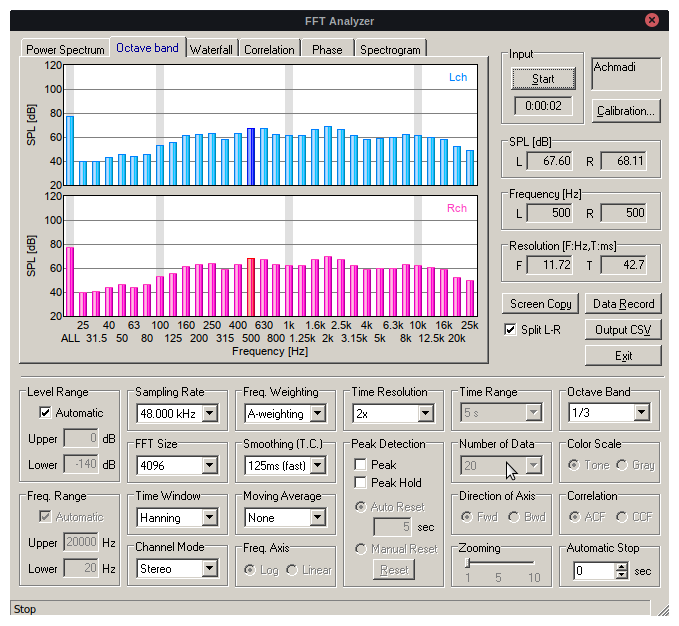
\includegraphics[width=300pt]{images/kemar/fft}
		\caption{Octave band pada FFT analyzer}
	\end{figure}
	
	Pada tampilan Octave-Band, klik satu bar frekuensi untuk mengetahui nilai SPL (dB)
	yang terisolasi dengan frekuensi lain.
	
	\newpage
	\subsubsection{Test Tone-Generation}
	Berikut adalah prosedur untuk mencoba \textit{tone-generation}:
	\begin{enumerate}
		\item Nyalakan unit prototype dan tunggu standby.
		Pastikan USB belum terhubung ke komputer.
		\item Sambungkan unit dengan headphone yang disiapkan
		\item Sambungkan USB ke komputer
		\item Cek nomor COM port pada Device manager
		\item Jalankan Hercules terminal
		\item Atur nama port sesuai COM port
		\item Klik \textbf{Open} pada Hercules terminal
		\item Masukkan perintah berikut:
		\begin{minted}[frame=lines,framesep=2mm,fontsize=\small]{text}
		out 500 5
		\end{minted}
		\item Setelah tekan (\keys{\return}), maka pada salah satu headphone
		akan membangkitkan tone selama kurang lebih 5detik.
		\item Jika setelah selesai, tekan \textbf{Close} pada terminal,
		lepas USB, dan matikan unit prototype.
		
	\end{enumerate}
	
	\subsubsection{Perintah yang Tersedia}
	
	Berikut beberapa perintah yang dapat diinputkan ke unit prototype:
	
	\begin{itemize}
		\item \textbf{test}.
		Perintah ini untuk mencoba headphone dengan mengeluakan tone singkat kanan-kiri bergantian.
		Perintahnya adalah (diakhiri (\keys{\return})):
		\begin{minted}[frame=lines,framesep=2mm,fontsize=\small]{text}
test
		\end{minted}
		
		\item \textbf{info}.
		Perintah ini untuk menampilkan informasi platform.
		Dapat digunakan sebagai perintah uji untuk melihat serial dan chip sudah berkerja atau tidak.
		Perintahnya adalah (diakhiri (\keys{\return})):
		\begin{minted}[frame=lines,framesep=2mm,fontsize=\small]{text}
info
		\end{minted}
		
		\item \textbf{out}.
		Perintah untuk membangkitkan tone dengan frekuensi dan skala yang diinginkan selama 5detik.
		Perintah adalah perintah utama dalam proses pengujian ini.
		Pola perintahnya adalah (diakhiri (\keys{\return})):
		\begin{minted}[frame=lines,framesep=2mm,fontsize=\small]{text}
out <frekuensi> <amplitudo>
		\end{minted}
		dengan:
		\begin{itemize}
			\item frekuensi adalah nilai frekuensi (dalam Hz) antara 250 sampai 8000.
			\item amplitudo adalah skala amplitudo antara 1 sampai 9
		\end{itemize}
		Contoh untuk tone 500Hz pada skala amplitudo 6 (diakhiri (\keys{\return})):
		\begin{minted}[frame=lines,framesep=2mm,fontsize=\small]{text}
out 500 6
		\end{minted}
	\end{itemize}
	
	\newpage
	\subsubsection{Troubleshoot}
	
	Berikut beberapa masalah yang terkadang sering muncul:
	\begin{enumerate}
		\item Perintah serial tidak merespon apapun kecuali hanya menampilkan prompt seperti:
		\begin{minted}[frame=lines,framesep=2mm,fontsize=\small]{text}
ch>
		\end{minted}
		Ini bukanlah masalah melainkan hanya respon saat baru selesai startup.
		Solusinya cukup masukkan perintah yang diinginkan sekali lagi.
		
		\item Serial USB tidak terdaftar pada \textit{Device-Manager}.\\
		Kemungkinan sumber masalah:
		\begin{itemize}
			\item Kabel USB tidak tersambung baik atau tidak menyediakan jalur data D+/D-.\\
			\textbf{Solusi}: ganti kabel USB
			
			\item Kabel USB terhubung ke komputer sebelum unit nyala dan standby.\\
			\textbf{Solusi}: lepas kabel USB dari komputer kemudian matikan dan nyalakan ulang unit.
			Setelah standby maka baru disambungkan ke komputer.
		\end{itemize}
		
		\item Unit prototype frezze atau hank.\\
		Ditandai dengan LED yang tidak lagi berkedip bergantian atau perintah serial tidak lagi merespon.\\
		Kemungkinan sumber masalah adalah kondisi \textit{race} pada threading dan interrupt.\\
		\textbf{Solusi}: lepas kabel USB dari komputer kemudian matikan dan nyalakan ulang unit.
		Setelah standby maka baru disambungkan ke komputer.
	\end{enumerate}
	
	\newpage
	\subsection{Pengujian}
	
	\subsubsection{Background}
	
	Sebelum melakukan sesi pengukuran, maka diperlukan mengambil profil bising ruangan.
	Dalam pengukuran ini, headphone telah terpasang pada KEMAR namun unit prototype dalam kondisi tidak menyala.
	Hasil pengukuran ini akan digunakan sebagai acuan pembanding hasil pengukuran.
	
	\subsubsection{Hasil}
	
	Hasil yang diharapkan adalah tabel SPL (dB) untuk setiap matrik frekuensi dan skala amplitudo.
	Dengan hasil tabel ini maka diharapkan ada acuan untuk pengaturan unit prototype sesuai standar yang digunakan pada nantinya.
	
	Berikut contoh tabel yang diharapkan:
	
	\begin{center}
		\begin{tabular}{|c|c|c|c|c|c|c|c|c|c|}
			\hline
			Fq/Ap & 9 & 8 & 7 & 6 & 5 & 4 & 3 & 2 & 1\\ [0.5ex]
			\hline\hline
			250Hz & X dB & X dB & X dB & X dB & X dB & X dB & X dB & X dB & X dB\\
			\hline
			500Hz & X dB & X dB & X dB & X dB & X dB & X dB & X dB & X dB & X dB\\
			\hline
			1000Hz & X dB & X dB & X dB & X dB & X dB & X dB & X dB & X dB & X dB\\
			\hline
			2000Hz & X dB & X dB & X dB & X dB & X dB & X dB & X dB & X dB & X dB\\
			\hline
			4000Hz & X dB & X dB & X dB & X dB & X dB & X dB & X dB & X dB & X dB\\
			\hline
			8000Hz & X dB & X dB & X dB & X dB & X dB & X dB & X dB & X dB & X dB\\
			\hline
		\end{tabular}
	\end{center}
	
	Tabel dalam format Excel 2003 (xls) dapat didownload di \url{https://intip.in/UjiAudiometri}.
	Untuk saat ini abaikan frekuensi 16kHz.
	
	\subsubsection{Perintah Serial}
	
	Perintah serial yang digunakan sebagaimana telah dijelaskan pada bab sebelumnya adalah perintah \textbf{out},
	dengan pola perintah:
	\begin{minted}[frame=lines,framesep=2mm,fontsize=\small]{text}
out <frekuensi> <amplitudo>
	\end{minted}
	dengan:
	\begin{itemize}
		\item frekuensi adalah nilai frekuensi (dalam Hz) mulai 250, 500, 1000, 2000, 4000, dan 8000.
		\item amplitudo adalah skala amplitudo pada nilai 1, 2, 3, 4, 5, 6, 7, 8, dan 9.
	\end{itemize}
	
	\newpage
	\subsubsection{Contoh Prosedur}
	
	Berikut adalah contoh prosedur untuk satu nilai uji pada satu frekuensi dan satu skala amplitudo.
	Sebagai contoh adalah frekuensi 1000Hz pada skala amplitudo 6.
	Sebelum pengujian, kembali cek ulang persiapan meliputi:
	\begin{itemize}
		\item Lakukan Pengukuran bising ruangan sebagai acuan pembanding.
		\item Nyalakan unit prototype. Pastikan LED biru menyala dan berkedip.
		\item Unit prototype telah standby dan terhubung laptop via USB.
		\item Serial terminal telah bisa mengirim perintah dan mendapat respon.
		\item Headphone telah terpasang ke unit uji KEMAR dan terhubung unit prototype.
		\item Komputer dan unit KEMAR sudah terhubung dengan Audio Capture Device.
		\item Real-Time Analyzer pada window FFT Octave-band telah terkalibrasi dan sudah start.
	\end{itemize}
	
	Berikut contoh prosedur satu nilai:
	\begin{enumerate}
		\item masukkan perintah tone untuk nilai frekuensi dan skala amplitudo yang ditentukan.
		Contoh (1000Hz skala 6):
		\begin{minted}[frame=lines,framesep=2mm,fontsize=\small]{text}
out 1000 6
		\end{minted}
		
		\item Tone akan dibangkitkan selama 5detik.
		
		\item Pada window Octave-band, klik bar pada frekuensi 1000Hz.
		
		\begin{figure}[!ht]
			\centering
			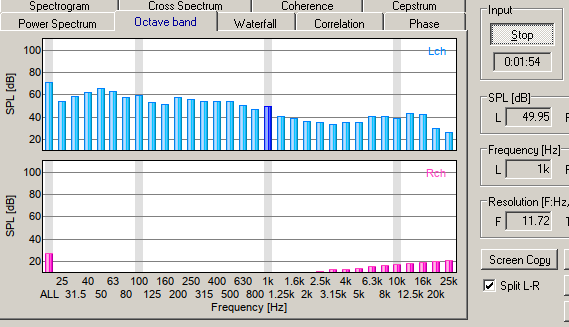
\includegraphics[width=300pt]{images/terminal/contoh}
			\caption{Contoh Nilai Uji}
		\end{figure}
		
		Terlihat bahwa nilai hasil uji adalah 49.95 dB (atau 50dB).\\
		\textbf{Catatan}: Contoh gambar di atas dilakukan pada ruangan biasa dengan penuh gangguan.
		
		\item Catat nilai SPL tersebut pada tabel Hasil sesuai frekuensi dan skala amplitudo
		
		\item Setelah 5detik, tone akan berhenti.
		
		\item Pengujian dapat dilanjutkan pada kombinasi frekuensi dan skala amplitudo lainnya.
	\end{enumerate}

	\newpage
	\subsubsection{Uji Konsistensi: Histeresis}
	
	Untuk uji histeresis, pada dasarnya adalah mengulang pengujian dengan membalik urutan skala output.
	Sebagai contoh:
	\begin{itemize}
		\item Pengujian telah dilakukan dengan skala output naik mulai dari 1 hingga 9 di setiap frekuensi.
		\item Pengujian selanjutanya dilakukan skala output turun mulai dari 9 hingga 1 di setiap frekuensi.
	\end{itemize}
	
	Dengan kedua proses di hari atau jam yang sama, maka disini diasumsikan daya baterai belum berubah signifikan.
	
	\subsubsection{Uji Konsistensi: Daya Baterai}
	
	Untuk uji baterai, maka dilakukan pengulangan uji seperti sebelumnya namun dengan hari yang berbeda.
	Selama unit tidak di-recharge, maka dengan memperhatikan:
	\begin{itemize}
		\item arus kerja chip STM32F401RE
		\item arus kerja chip MAX98357A
		\item arus kerja regulator TP0645
	\end{itemize}
	maka dapat diasumsikan bahwa daya baterai telah berkurang saat pengujian dibandingkan 1x24 jam sebelumnya.
	Selanjutnya dapat dilakukan pengujian ulang sebagaimana panduan sebelumnya.
	
	\subsubsection{Jumlah Hasil}
	Jumlah hasil tabel yang diharapkan dengan memperhatikan
	\begin{itemize}
		\item Headphone 2 unit (Bose dan Miniso)
		\item Unit prototype 2 unit (telah diberi Label A dan B)
		\item Pengujian histeris 2 kali (skala amplitudo naik dan turun)
		\item Pengujian 2 kali dengan perbedaan daya baterai (selisih setidaknya 1 hari)
	\end{itemize}
	
	maka diharapkan akan ada 16 tabel hasil di akhir pengujian.
	
	\vspace{30pt}\centering \textbf{--- Selesai ---}
	
	
\end{document}
